\documentclass{article}


\usepackage{arxiv}
\usepackage{authblk}
\usepackage{cite}
\usepackage[utf8]{inputenc} % allow utf-8 input
\usepackage[T1]{fontenc}    % use 8-bit T1 fonts
\usepackage{hyperref}       % hyperlinks
\usepackage{url}            % simple URL typesetting
%\usepackage[hyphens]{url}
\PassOptionsToPackage{hyphens}{url}\usepackage{hyperref}
\usepackage{booktabs}       % professional-quality tables
\usepackage{amsfonts}       % blackboard math symbols
\usepackage{nicefrac}       % compact symbols for 1/2, etc.
\usepackage{microtype}      % microtypography
\usepackage{lipsum}
\usepackage{subfig}
\usepackage{graphicx}
\graphicspath{ {./images/} }


\title{Contributions of the Petabyte Scale Sequence Search Codeathon toward efforts to scale sequence-based searches on the SRA}


\author[1]{A. Author}
\author[2]{B. Author}
\author[3]{C. Author}
%\author[2]{Corresponding Author\thanks{email@2nduniversity.com}}
\affil[1,2]{Author Affiliation 1}
\affil[3]{Author Affiliation 2}
{
    \makeatletter
    \renewcommand\AB@affilsepx{: \protect\Affilfont}
    \makeatother

    \affil[ ]{Email ids}

    \makeatletter
    \renewcommand\AB@affilsepx{, \protect\Affilfont}
    \makeatother

    \affil[1]{aa@x.gov}
    \affil[2]{ba@y.gov}
    \affil[1,3]{ca@z.gov}
}

\begin{document}
\maketitle
\begin{abstract}

The volume of biological data being generated by the scientific community is growing exponentially, reflecting technological advances and research activities. This increase in available data has great promise for pushing scientific discovery but also introduces new challenges that scientific communities need to address. The National Institutes of Health’s (NIH) Sequence Read Archive (SRA), which is maintained by the National Library of Medicine’s National Center for Biotechnology Information (NCBI), is a rapidly growing public database that researchers use to improve scientific discovery across all domains of life. As part of the Science and Technology Research Infrastructure for Discovery, Experimentation, and Sustainability (STRIDES) Initiative, over 40 petabytes of “next generation” (raw and SRA-formatted) sequencing data is accessible to anybody via two cloud service providers.

To help address the challenges of conducting large-scale analysis of omic data in the SRA and similar databases, the Department of Energy (DOE) Office of Biological and Environmental Research (BER), the NIH Office of Data Science Strategy (ODSS), and NCBI, held a virtual codeathon 'Petabyte Scale Sequence Search: Metagenomics Benchmarking Codeathon' on September 27 - Oct 1 2021, to address emerging Solutions in Petabyte Scale Sequence Search. The codeathon  attracted experts from national laboratories including the Los Alamos National laboratory (LANL), research institutions including the Joint Genome Institute (JGI) and students from universities across the world to develop benchmarking approaches to address challenges in conducting large-scale analyses of metagenomic data.

\end{abstract}


% keywords can be removed
%\keywords{First keyword \and Second keyword \and More}


\section{Introduction}
\label{sec:intro}

The revolution in next-generation nucleotide sequencing has provided profound insights into the genetic composition and variation within biological samples and has yielded a number of scientific breakthroughs including <<pick your favorite examples>>. This scientific work has been supported by investments in fundamental research, technology and infrastructure and the resultant decrease in nucleotide sequencing and data storage costs have led to an exponential increase in the volume of sequence data generated by the scientific community. 
%<<Include some examples of exciting scientific work that relies on sequence data here to draw folks in>>

\subsection{The NIH Sequence Read Archive has reached the petabyte scale}
\label{sec:SraGrowth}

The Sequence Read Archive (SRA) at the National Institutes of Health is a diverse collection of next generation nucleotide sequencing data hosted by the National Center for Biotechnology (NCBI) at the National Library of Medicine (1,2). SRA provides a repository where data creators can share their raw sequence data with the scientific community and holds both public data available to all researchers and controlled access data derived from human research studies for use by qualified biomedical investigators who agree in advance to use the data appropriately. Sequence data in the archive is linked to associated metadata that provides information about the sequenced sample and can be used to associate genetic information in SRA with phenotypic, clinical, and environmental attributes [cite] \cite{katz2021stat}. The archive is also part of the International Nucleotide Sequence Database Collaboration (INSDC), and SRA sequence data and associated metadata as well as analogous data submitted to the European Nucleotide Archive (ENA) are exchanged among member databases.

\begin{figure}[t]
        \centering
        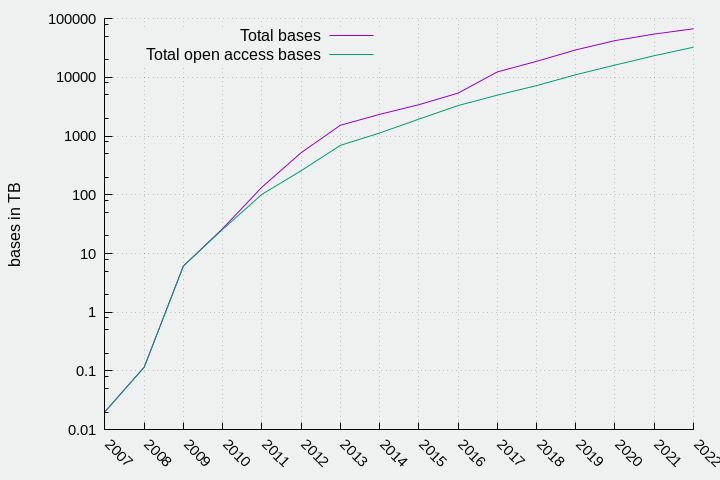
\includegraphics[width=0.6\textwidth]{images/sra_bases_TB.png}
        \caption{Growth of SRA. Databases like the NIH Sequence Read Archive are growing rapidly and are used extensively by scientific communities. As these databases grow, so do their potential scientific value, but work must be done to ensure ease of access.}
        \label{fig:sragrowth}
\end{figure}

The growth in nucleotide sequencing data within the scientific community has led to an explosion in the size of SRA (as seen in Figure 1 \ref{fig:sragrowth}), 
%Do we additional updates to Figure 1??
and there are now more than 16.8 million submitted samples from across all the domains of life that together comprise more than 17 petabytes of raw sequencing data in the repository (1,2). Given its vast size and diversity, the SRA represents a crucial resource for the scientific community, and researchers have developed bioinformatic tools and methods and tools that support deep analysis of SRA data – everything from assembly and annotation of genomes, characterization of human pathogens, discovery of novel organisms and viruses, and association of genetic signatures from complex microbiome and metagenomic samples with environmental attributes, to prediction of the functional significance of rare human genetic variation [cites].

To sustain future growth and facilitate expanded use the petabyte-scale SRA dataset, NIH partnered with Google Cloud Platform (GCP) \cite{GCP} and Amazon Web Services (AWS) \cite{AWS} in 2019, through the NIH Science and Technology Research Infrastructure for Discovery, Experimentation, and Sustainability (STRIDES) Initiative \cite{stridesini}. This partnership was part of a larger NIH STRIDES effort to build a cloud-enabled biomedical dataverse, with new processes, tools, and architecture to drive development of an equitable ecosystem that makes NIH-funded data findable, accessible, interoperable, and reusable (FAIR) \cite{wilkinson2016fair}. The entirety of the SRA sequence dataset is now replicated on Google and Amazon cloud platforms, and associated BioProject, BioSample, and SRA metadata is available through Google Big Query and Amazon Athena services. The public SRA dataset is available in normalized format through the AWS Open Data Program, and data can be egressed without charge into cloud and local locations \cite{sracosts}. 
%Is this a good place for talking about the cloud in terms of storage, access, and compute or should this go into a separate section?

\subsection{Petabyte-scale sequence search will improve the scientific impact of SRA}
\label{sec:psss}

While staging on cloud platforms provides enhanced access to SRA, successful use of the archive will require the basic ability to search across the petabyte-scale dataset to locate samples of interest. Search in this context can be thought of as two discrete functions: (1) text-based search, where queries to are matched to metadata descriptors associated with deposited sequence samples, and (2) sequence-based search, where sequence strings are matched to the sequence content of a sample. Attribute-based search depends on accurate sample metadata and is hindered by missing, incorrect, or inconsistently labeled or formatted metadata [3 plus other cites]. In contrast, sequence-based search is essentially agnostic to the sample information provided by data submitters and depends instead on the content of the sequence data itself.

Sequence-based search was critical to the application of GenBank as a public genetic sequence repository. The Basic Local Alignment Search Tool (BLAST) provided a way for researchers to compare experimentally derived sequences to those in the GenBank and to identify sequences of interest, such as [~2 EXAMPLES] [cites]. BLAST now supports sequence-based searches using nucleotide and protein sequences, translated sequences, and sequence models.These different search modalities support the identification of sequences with extensive homology to the query as well as the identification of more divergent sequences.  Similar search functionality will be critical to the usability of SRA On one hand, the immense scale of the database (? times the size of GenBank) imposes unique challenges to sequence search tools. On the other hand, the same scale will provide unique scientific rewards if such tools are successfully implemented.

\subsubsection{The value of sequence-based search }
\label{sec:SeqSearch}

Recent work by the Serratus group demonstrates the potential of SRA-wide sequence search to identify novel viruses \cite{edgar2022petabase}. However,no extant tool supports easy search across , one size fits all approach to sequence based search, and search strategies vary with the specific use case and underlying data. In some cases exact nucleotide matches are desired, so that samples that include specific query sequences can be identified. In other cases, similar matches to the query are desired, like when searching for samples that include homologous genes or related organisms. These different use cases often require different technical solutions, and in the case of BLAST, different databases and algorithms are constructed to support explicit and domain based nucleotide and amino acid sequence searches [cite]. Therefore it is likely that different scientific domains will require different computational tools capable of searching SRA at the petabyte scale.

% Should there be another subsection here on "Recent studies using the Serratus"??

\subsubsection{Metadata Challenges }
\label{sec:MetadataChallenges}

When the scientist’s goal is discovery of what relevant data might be available in the repository, a direct search on sequence data circumvents issues with missing or inaccurate metadata. Improving the accuracy of metadata is challenging and is an active area of research and is outside the scope of this investigation. Tools such as Metaseek aggregate the SRA metadata and preliminary investigation shows that many SRA entries are incomplete. We are interested in the types of discovery that are possible if scientists can quickly determine all the datasets that contain a particular gene or genome. The metadata associated with those datasets may be inaccurate and that will decrease the utility in reusing that data. Current advances in the area of large language models may yield improvements in language alignment that make metadata-based search strategy more powerful by improving current and future metadata quality. 

\begin{figure}%
    \centering
    \subfloat[\centering Percent public SRA accessions by organism]{{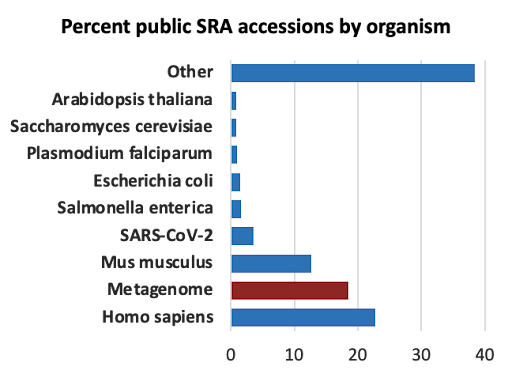
\includegraphics[width=7cm]{images/SRA_acc_organism.png} }}%
    \qquad
    \subfloat[\centering Percent public SRA accessions downloaded]{{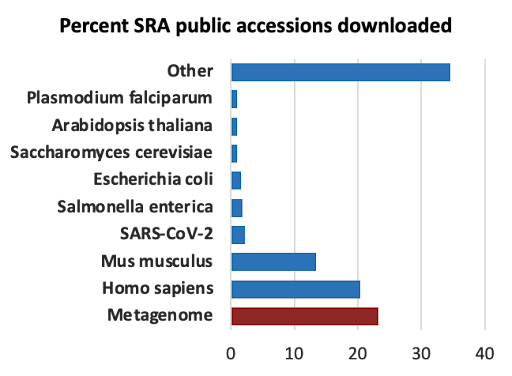
\includegraphics[width=7cm]{images/SRA_public_acc_downloaded.png} }}%
    \caption{SRA metagenomic accessions and usage}%
    \label{fig:metagenomicsradata}%
\end{figure}

\subsection{Metagenomics}
\label{sec:MetagenomicsData}

A metagenome is a dataset that represents a collection of genomes found in a sample. The sample may be from the human gut, a marine estuary, exotic locations, or your office. The study of the microbial communities is important because many phenomena are driven not just by the actions of a single microbial species, but many working together. Metagenomes are large, complex, and challenging to analyze, the largest dataset sizes are on the O(10TB). The field has benefited from a reduction in sequencing costs, as well as, more sophisticated data processing and analysis techniques that has led to an increase in the number of metagenomic studies. The number and size of metagenomic datasets being deposited and utilized in SRA is growing at a faster rate than other datasets.

\begin{itemize}
    \item SRA… and a large percentage of SRA data usage as seen in Figure \ref{fig:metagenomicsradata}
    \item Metagenomic datasets provide a unique set of challenges that include both known and unknown organisms within a sample
    \item Ability to identify organismal content and/or correlate it with sample attributes critical to use of metagenomic sequence datasets

\end{itemize}

\subsubsection{Examples of scientific inquiries/discoveries based on metagenomic analysis}
\label{sec:ExamplesOfMetadatAnalysis}

Challenge: as datasets get larger, and with long-read seq data, get more complete discrete genomes out. Especially w/ highly complex env samples. Can you leverage across existing sequence space to simplify the problem.




\section{Current approaches to sequence search}
\label{sec:SeqSearchApproches}

Sequence-based searches attempt to match a sequence string query to a target sequence within the search set. Queries can vary in sequence length as well as the identity between query and intended search targets depending on use cases that range from identifying samples with targets that generally match a genome-sized query to identifying sequences that are similar to conserved domain within a gene to explicitly matching sets of nucleotide variations. A variety of approaches have been developed to search SRA data, alignment, indexing, suffix arrays, model-based approaches (HMMER, neural nets, etc.) (7,8),  and others. Tools that implement indexing and/or alignment based strategies that will be the focus here. 

\subsection{Alignment-based searches}
\label{sec:AlignmentBased}

Sequence alignment is a method that positions the biological sequences’ building blocks to identify regions of similarity that may have consequences for functional, structural, or evolutionary relationships. In the 80s and 90s many alignment-based methods were developed to help researchers make sense of next-generation sequence data. Some of the most well-known alignment tools are BLAST, Smith-waterman, BLAT, etc. The BLAST tools are still the most popular ways to execute a search on many web-based biological platforms (EBI, IMG, Phytozome, etc). There have been advances in improving the computational efficiency of the aligners, however, there are trade-offs in efficiency, sensitivity, and accuracy. Alignment is still irreplaceable in many aspects of today's biology, such as the annotation of conserved protein domains and motifs, tracking phenotype-related sequence polymorphisms, reconstruction of ancestral DNA sequences, determining the rate of sequence evolution, and homology-based modeling of three-dimensional protein structures, all of which require highly sensitive matching.

\subsection{Index-based searches}
\label{sec:IndexBased}

Performing alignment-based sequence-level searches on large collections of SRA and WGS data can quickly become impractical due to size of the databases. For instance, given a query sequence, searching across all metagenomes in the SRA would entail a BLAST search against >3.2 million (~2 PB of data) accessions.  Such searches are not only hard to scale due to the significant memory and time footprint, but can be infeasible when searching across the entire database. As a result, users will have to limit their searches based on attributes such as taxonomy, metadata, sequencing platform etc. Alternatively, several index-based approaches break the search space down to short non-overlapping sequence strings of a fixed length called “k-mers”. These k-mers are then associated either directly with the sample from which they originated or with organisms or other biological markers in the sample and stored in an index. The query sequence is broken down into overlapping k-mers of the same length that are then used to “look up” samples that include matching k-mers, organisms, or biological markers. Notable examples for the index-based approach include BIGSI (BItsliced Genomic Signature Index)[18], Soumash/Branchwater [22-24], Pebblescout [20], Kraken[15,16], STAT[17].

\subsection{Alignment-based vs Index-based comparison}
\label{sec:compareSeqMethods}

Index and alignment methods each have their own advantages and disadvantages:
\begin{itemize}
    \item Index searches provide potentially rapid search across many targets
    \item Index searches are dependent on the representation of the search space and are influenced by the density of target sequence sampling 
    \item Index searches typically require exact matches between query and target, which could limit their sensitivity to diverged sequences
    \item Indexes used to support search can be very large, but there are approaches to reduce size (min-hash, sequential indexes, bloom filters)
    \item Index based approaches require the index to grow incrementally as new sequences (assembled or unprocessed) are deposited. Depending on the organism, there can be enormous diversity (eg. viruses) which could limit scaling the index.
    \item Alignment methods allow for mismatches between query and target providing a mechanisms for identifying related, but not exact matches to the query
    \item Existing alignment methods also support model based queries
    \item Alignment methods can be computationally expensive as well as memory intensive
    \item Performance metrics of index and alignment based methods
Can we include metrics around size (index tables vs alignment dbs) and performance (lookup vs linear vs quadratic)
    \item Index-based and alignment-based methodologies are not mutually exclusive. Index-based methods can be used to reduce the search space prior to attempting to build alignments. In practice k-mer lookups are used to reduce the sequence search space 
    \item Transition to scaling section - All of these issues will be exacerbated by the continued growth of data generation. A focused community-based approach is crucial to identifying a path toward more accessible and usable sequence data archives. 

\end{itemize}

\section{Challenges for large-scale sequence search}
\label{sec:SeqSearchChallenges}

Data repositories are growing constantly, so as soon as an index is created, it is out of date. Similarly, as the repository’s size increases, alignment-based approaches become too expensive. There are fundamental limitations to each approach explored in the codeathon, however, these approaches also represent the best tools available for a problem that must be addressed to maintain the usability of the Sequence Read Archive. 
A scientist conducts a search for data because they need it to support an experiment or inquiry. Different scientific questions may require different indexes of the sequence data or flexible workflows to set up a series of steps that filter and refine their search. The concept of search must be expanded to include not just SQL-style queries optimized for joining metadata, but fast analysis tools that allow a user to reconfigure data structures on the fly to look for relationships. Refinement of search-based workflows yields insights into the strengths and weaknesses of different components, and can pinpoint where resources should be invested. 
Working directly with the raw reads, while challenging, avoids potential issues created by inconsistent data processing. For example, large fractions of metagenomic datasets do not assemble into contigs, so a comprehensive search of information from those samples must be done at the read level. 
Exploration of sequence data is amenable to a hybrid indexing and alignment approach where the inexpensive indexes can be calculated and used to reduce the search space for the more costly and sensitive alignment methods. 

\paragraph{Challenges with clustering:}
-Costs of building the clustered database and dealing with iterative updates
- Clustering is very difficult for metagenomes- you always end up with sequences that are not clusterable- do you throw them away, do you keep them; what do you do?
- At what level do you cluster?? Kmer, read, contig, nucleotide, amino acid, etc.…?  The clustering might need to be catered to the type of sample you have: A metagenome, which is complex and has sparse coverage, might need to be clustered differently than a less complex sample like a single organism where you have way higher coverage across the entire genome
-Defining the meaningful pieces of sequences (it’s like defining what “words” are in natural language processing) and the attributes that make up the semantic space. 
-Compressing search space using current biological knowledge is problematic for metagenomes, which have a lot of diversity; for example, if you align at the protein level, you might only get ~50\% of your reads aligned to known proteins- then what do you do with the rest of the reads?  Also, this approach is based on current biological knowledge, which is likely incomplete; one panelist was “worried about “pouring concrete” on our current understanding of biology if we set up our scientific searches to implicitly depend on current assumptions.”

\section{The Metagenomics Benchmarking Codeathon}
\label{sec:psss-codeathon}

The National Institutes of Health (NIH) Office of Data Science Strategy (ODSS), the National Library of Medicine’s (NLM’s) National Center for Biotechnology and Information (NCBI), and the Department of Energy’s (DOE’s) Office of Biological and Environmental Research (BER) hosted scientists from around the world to participate in a virtual Petabyte-Scale Sequence Search: Metagenomics Benchmarking Codeathon. The codeathon, held September 27-October 1, 2021, attracted experts from national laboratories including the Los Alamos National laboratory, research institutions including the Joint Genome Institute, and students from universities across the world to develop benchmarking approaches to address challenges in conducting large-scale analyses of metagenomic data.

To take advantage of this growing collection of biomedical data, there is a need for efficient methods to search the archive using nucleotide sequences. Just as the introduction of tools like Basic Local Alignment Search Tool (BLAST) provided a key to unlock the potential of the GenBank archive, similar approaches are needed for SRA. Towards these efforts, we have developed an interagency Emerging Solutions in Petabyte Scale Sequence Search (ESPSSS) initiative which hosted its first workshop in June. Explaining the impetus for the workshop, Dr. Susan Gregurick, NIH Associate Director for Data Science and ODSS Director, said: “{\it We all share a common problem and a need to develop, enhance, and implement methods that streamline data access, search or findability, and ultimately data reuse}.” Dr. Todd Anderson, the Biological Systems Science Division Director from the DOE, added that “{\it There is much to be gained from employing big data technology to assist with experimentation in biological sciences}.”

As metagenomic samples comprise more than 30\% of the sequence records in SRA, ESPSSS is initially focusing on metagenomic benchmarking. In the spirit of developing community driven solutions, ESPSSS hosted the virtual Petabyte-Scale Sequence Search: Metagenomics Benchmarking Codeathon in September to bring together students, researchers, and computing professionals to collaborate on developing sequence search benchmarking approaches.
Collaborative work by codeathon participants—who were split into four teams— generated the following proof-of-concept or early-stage solutions:
\begin{enumerate}
    \item a pipeline used for the identification of metagenomic samples with user-provided long sequence queries,
    \item a gold-standard dataset and pipeline to benchmark contig containments,
    \item a benchmark harness for read/contig tools, and
    \item a pipeline to combine an experimental SRA sequence index with BLAST.
\end{enumerate}



%\clearpage

\section*{Acknowledgments}
This work was supported in part by the National Center for Biotechnology Information of the National Library of Medicine (NLM), National Institutes of Health.



%\bibliographystyle{unsrt}  
%\bibliography{references}  %%% Remove comment to use the external .bib file (using bibtex).
%%% and comment out the ``thebibliography'' section.


%%% Comment out this section when you \bibliography{references} is enabled.


\bibliography{references}

%This defines the bibliographies style. Search online for a list of available styles.
\bibliographystyle{abbrv}


\end{document}
